\documentclass{ees}

\newgeometry{twoside=false,left=20mm,right=40mm,top=20mm,bottom=40mm}

\newlist{bulletlist}{itemize}{1}
\setlist[bulletlist]{
  partopsep=0pt,
  parsep=0pt,
  itemsep=0pt,
  label=\textbullet
}

\setcounter{tocdepth}{1}
\DeclareTOCStyleEntry[
  indent=0pt,
  beforeskip=\baselineskip,
  entrynumberformat=\@gobble,
  entryformat=\sbseries,
  numwidth=2em,
  linefill=\hfill,
  pagenumberbox=\pnumbox,
  pagenumberformat=\sbseries
]{tocline}{chapter}


\begin{document}

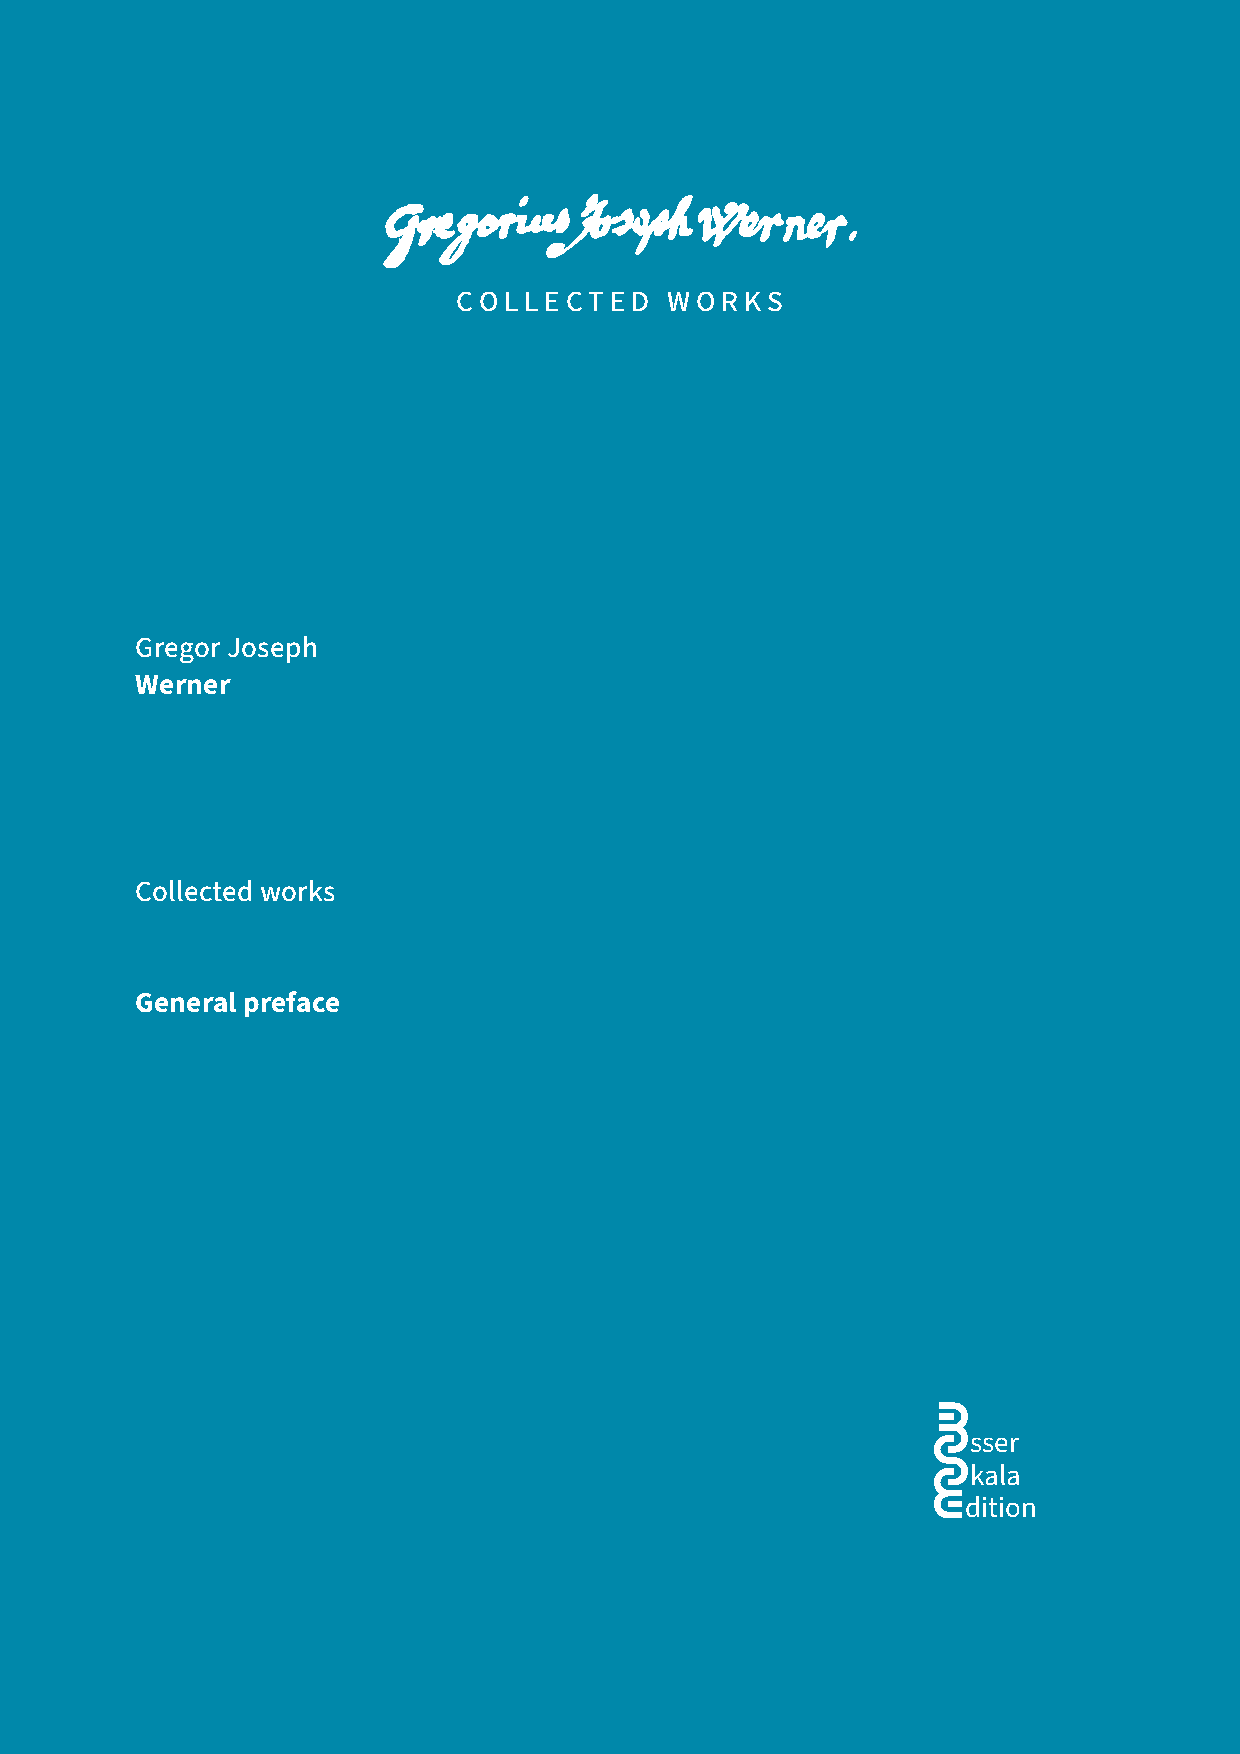
\includepdf{cover_general_preface.pdf}
\pagenumbering{arabic}
\setcounter{page}{1}

\tableofcontents

\chapter{General preface}

\textit{Gregor Joseph Werner: Collected works} (GJW:CW) is an edition project that will make Werner’s music available in modern editions.

For detailed information on Werner's works, we refer the reader to our thematic catalogue of works (\href{https://gregor-joseph-werner.at}{https://gregor-joseph-werner.at}), which is currently under development. WerW numbers are cited from this catalogue.


\section{Editorial guidelines}

In general, GJW:CW follows the \href{https://edition.esser-skala.at/about/editorial-guidelines/}{editorial guidelines} for the Edition Esser-Skala.

% Some peculiarities for editing Werner's works are highlighted below:

% \begin{bulletlist}
%   \item
% \end{bulletlist}


\section{Acknowledgements}

Assistance of the following people and institutions is gratefully acknowledged:
Thomas Dolezal (Dommusikarchiv Eisenstadt – A-Ed),
Peter Deinhammer (Benediktinerstift Lambach, Musikarchiv – A-LA),
Ilse Beel (Koninklijk Conservatorium Brussel, Bibliotheek – B-Bc),
Maria Šťastná (Knihovna Národního muzea, Praha – CZ-Pn and CZ-Pnm),
Gertraud Gaukesbrink (Santini-Bibliothek, Münster – D-MÜs),
Klaus Petermayr (Oberösterreichisches Landesmuseum, Musiksammlung),
as well as the staff of
the Österreichische Nationalbibliothek, Musiksammlung, Wien (A-Wn),
the Staatsbibliothek zu Berlin - Preußischer Kulturbesitz, Musikabteilung (D-B),
the Sächsische Landesbibliothek - Staats- und Universitätsbibliothek, Dresden (D-Dl),
the Universitäts- und Landesbibliothek Darmstadt, Musikabteilung (D-DS),
the Duke University Libraries, Music Library, Durham, NC (US-DMu),
and the Zentral- und Hochschulbibliothek Luzern (CH-Lz).


\clearpage
\markdownInput{../CHANGELOG.md}

\end{document}
